% ------------------------------------------------------------------------
% file `1_E_juin-transferer-22-exercise-body.tex'
%   in folder `xsim/'
%
%     exercise of type `transferer' with id `22'
%
% generated by the `transferer' environment of the
%   `xsim' package v0.21 (2022/02/12)
% from source `1_E_juin' on 2024/06/20 on line 535
% ------------------------------------------------------------------------
    Un club de sport va fêter ses 10 ans en septembre. Le secrétaire du club a rassemblé quelques données pour analyser l'évolution du club. \\ Réponds aux questions suivantes en observant le graphique.

    % \begin{tikzpicture}
    %     \begin{axis}[
    %             x tick label style={/pgf/number format/1000 sep=},
    %             ymin=0,
    %             ymax=160,
    %             xtick pos=left,
    %             ytick pos=left,
    %             ytick distance=10,
    %             ymajorgrids,
    %             y minor tick num =1,
    %             yminorgrids
    %         ]
    %         \addplot coordinates{
    %                 (2012,35)
    %                 (2013,40)
    %                 (2014,55)
    %                 (2015,60)
    %                 (2016,95)
    %                 (2017,115)
    %                 (2018,110)
    %                 (2019,120)
    %                 (2020,80)
    %                 (2021,120)
    %                 (2022,150)
    %             };
    %     \end{axis}
    % \end{tikzpicture}
\begin{center}
    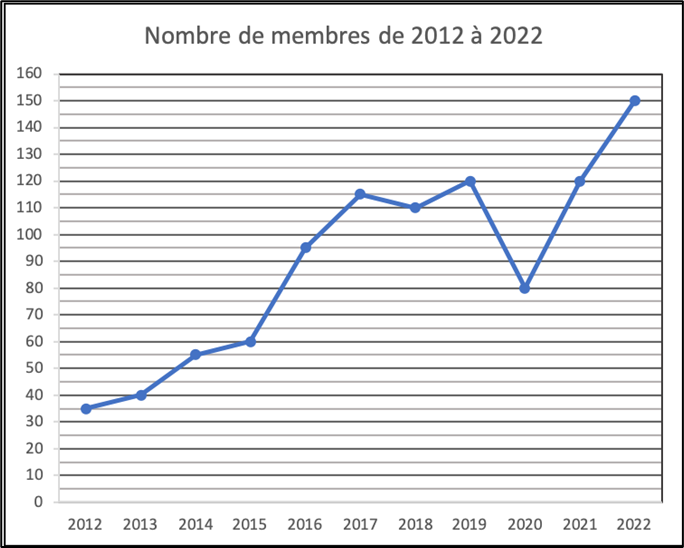
\includegraphics[width=\linewidth]{img/voitures.png}
\end{center}
        \begin{tasks}
            \task! Repasse à l'aide d'un fluo la partie du graphique qui montre la plus forte augementation des inscriptions.
            % \task En quelle année le nombre d'inscrits a-t-il le plus augmenté ?
            \task Cite deux années où le club a compté le même nombre de membres.
            \vspace{3em}
            \task Est-il vrai que le nombre d'inscrits a doublé entre 2015 et 2019 ? Laisse ta démarche visible.
        \end{tasks}
